% Headline metrics relative to the fno-21cm multi-field baseline (tbs+histtb).
% Numbers: CompAstro wiki, "Rhizome Neural Operator Results" §6.1, §6.7 (199 test cones).
% Build:  cd Figures/src && pdflatex metric_ratios.tex && mv metric_ratios.pdf ..
\documentclass[border=4pt]{standalone}
\usepackage[T1]{fontenc}
\IfFileExists{fourier.sty}{\usepackage{fourier}}{\usepackage{lmodern}}
\usepackage{amsmath}
\usepackage[dvipsnames]{xcolor}
\usepackage{pgfplots}
\pgfplotsset{compat=1.16}

\colorlet{c3d}{NavyBlue!55}
\colorlet{c2d}{ForestGreen!70!black}
\colorlet{cpw}{BurntOrange!85}

\begin{document}
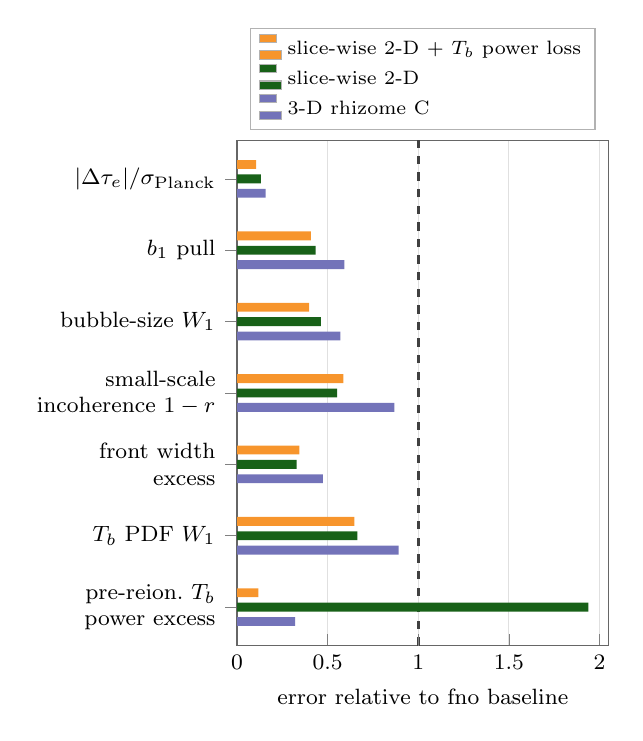
\begin{tikzpicture}
\begin{axis}[
    xbar, bar width=3.2pt,
    width=6.3cm, height=8.0cm,
    xmin=0, xmax=2.05, xtick={0,0.5,1,1.5,2},
    xlabel={error relative to fno baseline},
    xlabel style={font=\footnotesize},
    symbolic y coords={Tbpre,TbW1,front,incoh,bubble,b1,tau},
    ytick=data,
    yticklabels={
      {pre-reion.\ $T_b$\\power excess},
      {$T_b$ PDF $W_1$},
      {front width\\excess},
      {small-scale\\incoherence $1-r$},
      {bubble-size $W_1$},
      {$b_1$ pull},
      {$|\Delta\tau_e|/\sigma_{\mathrm{Planck}}$}},
    yticklabel style={font=\footnotesize, align=right},
    y dir=normal,
    enlarge y limits=0.09,
    tick label style={font=\footnotesize},
    xmajorgrids, grid style={black!12},
    legend style={font=\scriptsize, at={(0.5,1.02)}, anchor=south, draw=black!30, cells={anchor=west}},
    legend cell align=left,
    reverse legend,
    axis line style={black!60},
    ytick pos=left, xtick pos=bottom,
    every axis plot/.append style={draw=none},
    extra x ticks={1}, extra x tick labels={},
    extra x tick style={grid=major, major grid style={dashed, black!75, line width=0.9pt}},
  ]
  % 3-D rhizome C
  \addplot[fill=c3d] coordinates {
    (0.320,Tbpre) (0.891,TbW1) (0.474,front) (0.868,incoh) (0.570,bubble) (0.592,b1) (0.158,tau)};
  % slice-wise multi-field (plain)
  \addplot[fill=c2d] coordinates {
    (1.938,Tbpre) (0.664,TbW1) (0.329,front) (0.552,incoh) (0.463,bubble) (0.434,b1) (0.132,tau)};
  % slice-wise multi-field + T_b power loss
  \addplot[fill=cpw] coordinates {
    (0.117,Tbpre) (0.647,TbW1) (0.344,front) (0.586,incoh) (0.397,bubble) (0.408,b1) (0.105,tau)};
  \legend{3-D rhizome C, slice-wise 2-D, slice-wise 2-D + $T_b$ power loss}
\end{axis}
\end{tikzpicture}
\end{document}
